\chapter[Introdução]{Introdução}

\section{Motivação}

O estilo de redação deve atentar a boa prática da linguagem técnica. Para a 
terminologia metrological usar o Vocabulário Internacional de Termos 
Fundamentais e Gerais de Metrologia\cite{inmetro2003}  (Instituto Nacional de Metrologia, 
2003).

Grandezas dimensionais devem ser apresentadas em unidades consistentes com 
o Sistema Internacional de Unidades  (SI). Outras unidades podem ser usadas 
como unidades secundárias entre parenteses se necessário. Exceções são 
relacionadas a unidades não-SI usadas como identificadores comerciais como 
pro exemplo \lq\lq disquete de  3$\nicefrac{1}{2}$ polegadas\rq\rq. 

Na apresentação de números ao longo do texto usar virgula para separar a 
parte decimal de um número. Resultados experimentais devem ser apresentados 
com sua respectiva incerteza de medição.

\section{Títulos de capítulos e seções}

Recomendações de formatação de seções 

\begin{description}

	\item \textbf{1 SEÇÃO PRIMÁRIA - MAIÚSCULAS; NEGRITO; TAMANHO 12;}

	\item 1.1 SEÇÃO SECUNDÁRIA – MAIÚSCULAS; NORMAL; TAMANHO 12; 

	\item \textbf{1.1.1 Seção terciária - Minúsculas, com exceção da 
	primeira letra; negrito; tamanho 12;}

	\item 1.1.1.1 Seção quaternária - Minúsculas, com exceção da primeira 
	letra; normal tamanho 12; 

 	\item \textit{1.1.1.1.1 Seção quinária - Minúsculas, com exceção da 
	primeira letra; itálico; tamanho 12.}

\end{description}

\section{Notas de rodapé}

Notas eventualmente necessárias devem ser numeradas de forma seqüencial ao 
longo do texto no formato 1, 2, 3... sendo posicionadas no rodapé de cada 
página na qual a nota é utilizada.\footnote{Como, por exemplo, esta nota}

\section{Equações}

Equações matemáticas devem ser numeradas seqüencialmente e alinhadas a 
esquerda com recuo de 0,6 cm. Usar numerais arábicos entre parênteses, 
alinhado a direita, no formato Times New Roman de 9 pts. para numerara as 
equações como mostrado na Eq. (\ref{eqn01}).

Referências a equações no corpo do texto devem ser feitas como \lq\lq Eq. 
(\ref{eqn01})\rq\rq\ quando no meio de uma frase ou como \lq\lq Equação 
(\ref{eqn01})\rq\rq\ quando no inicio de uma sentença. Um espaçamento de 11 
pontos deve ser deixado acima, abaixo e entre equações subseqüentes. Para uma 
apresentação compacta das equações deve-se usar os símbolos e expressões 
matemáticos mais adequados e parênteses para evitar ambigüidades em 
denominadores. Os símbolos usados nas equações citados no texto devem 
apresentar exatamente a mesma formatação usada nas equações.
\begin{equation}
\label{eqn01}
	\frac{d\mathbf{C}}{dw} = \frac{du}{dw}\cdot \mathbf{F}_u + 
		\frac{dv}{dw}\cdot \mathbf{F}_v 
\end{equation}

O significado de todos os símbolos mostrados nas equações deve ser apresentado 
na lista de símbolos no inicio do trabalho, embora, em certas circunstancias o 
autor possa para maior clareza descrever o significado de certos símbolos no 
corpo do texto, logo após a equação.

\section{Figuras e Gráficos}

As figuras devem ser centradas entre margens e identificadas por uma legenda 
alinhada a esquerda com recuo especial de deslocamento de 1,8 cm, com mostrado 
na Fig. (\ref{fig01}). O tamanho das fontes empregadas nos rótulos e anotações 
usadas nas figuras deve ser compatível com o usado no corpo do texto. Rótulos e 
anotações devem estar em português, com todas as grandezas mostradas em 
unidades do SI (Sistema Internacional de unidades).

Todas as figuras, gráficos e fotografias devem ser numeradas e referidas no 
corpo do texto adotando uma numeração seqüencial de identificação. As figuras e 
gráficos devem ser claras e com qualidade adequada para eventual reprodução 
posterior tanto em cores quanto em preto-e-branco.

As abscissas e ordenadas de todos os gráficos devem ser rotuladas com seus 
respectivos títulos em português seguida da unidade no SI que caracteriza a 
grandes entre colchetes. 

A referência explícita no texto à uma figura deve ser feita como 
\lq\lq Fig. (\ref{fig01})\rq\rq\ quando no meio de uma frase ou como 
\lq\lq Figura (\ref{fig01})\rq\rq\ quando no início da mesma. Referencias 
implícitas a uma dada figura devem ser feitas entre parênteses como 
(Fig. \ref{fig01}). Para referências a mais de uma figura as mesmas regras 
devem ser aplicadas usando-se o plural adequadamente. Exemplos:

\begin{itemize}
	\item \lq\lq Após os ensaios experimentais, foram obtidos os resultados 
	mostrados na Fig. (\ref{fig01}), que ...\rq\rq
	\item \lq\lq A Figura (\ref{fig01}) apresenta os resultados obtidos, onde 
	pode-se observar que ...\rq\rq
	\item \lq\lq As Figuras (1) a (3) apresentam os resultados obtidos, 
	...\rq\rq
	\item \lq\lq Verificou-se uma forte dependência entre as variáveis citadas 
	(Fig. \ref{fig01}), comprovando ...\rq\rq
\end{itemize}

Cada figura deve ser posicionada o mais próxima possível da primeira citação 
feita à mesma no texto, imediatamente após o parágrafo no qual é feita tal 
citação, se possível, na mesma página.
\begin{figure}[h]
	\centering
	\label{fig01}
		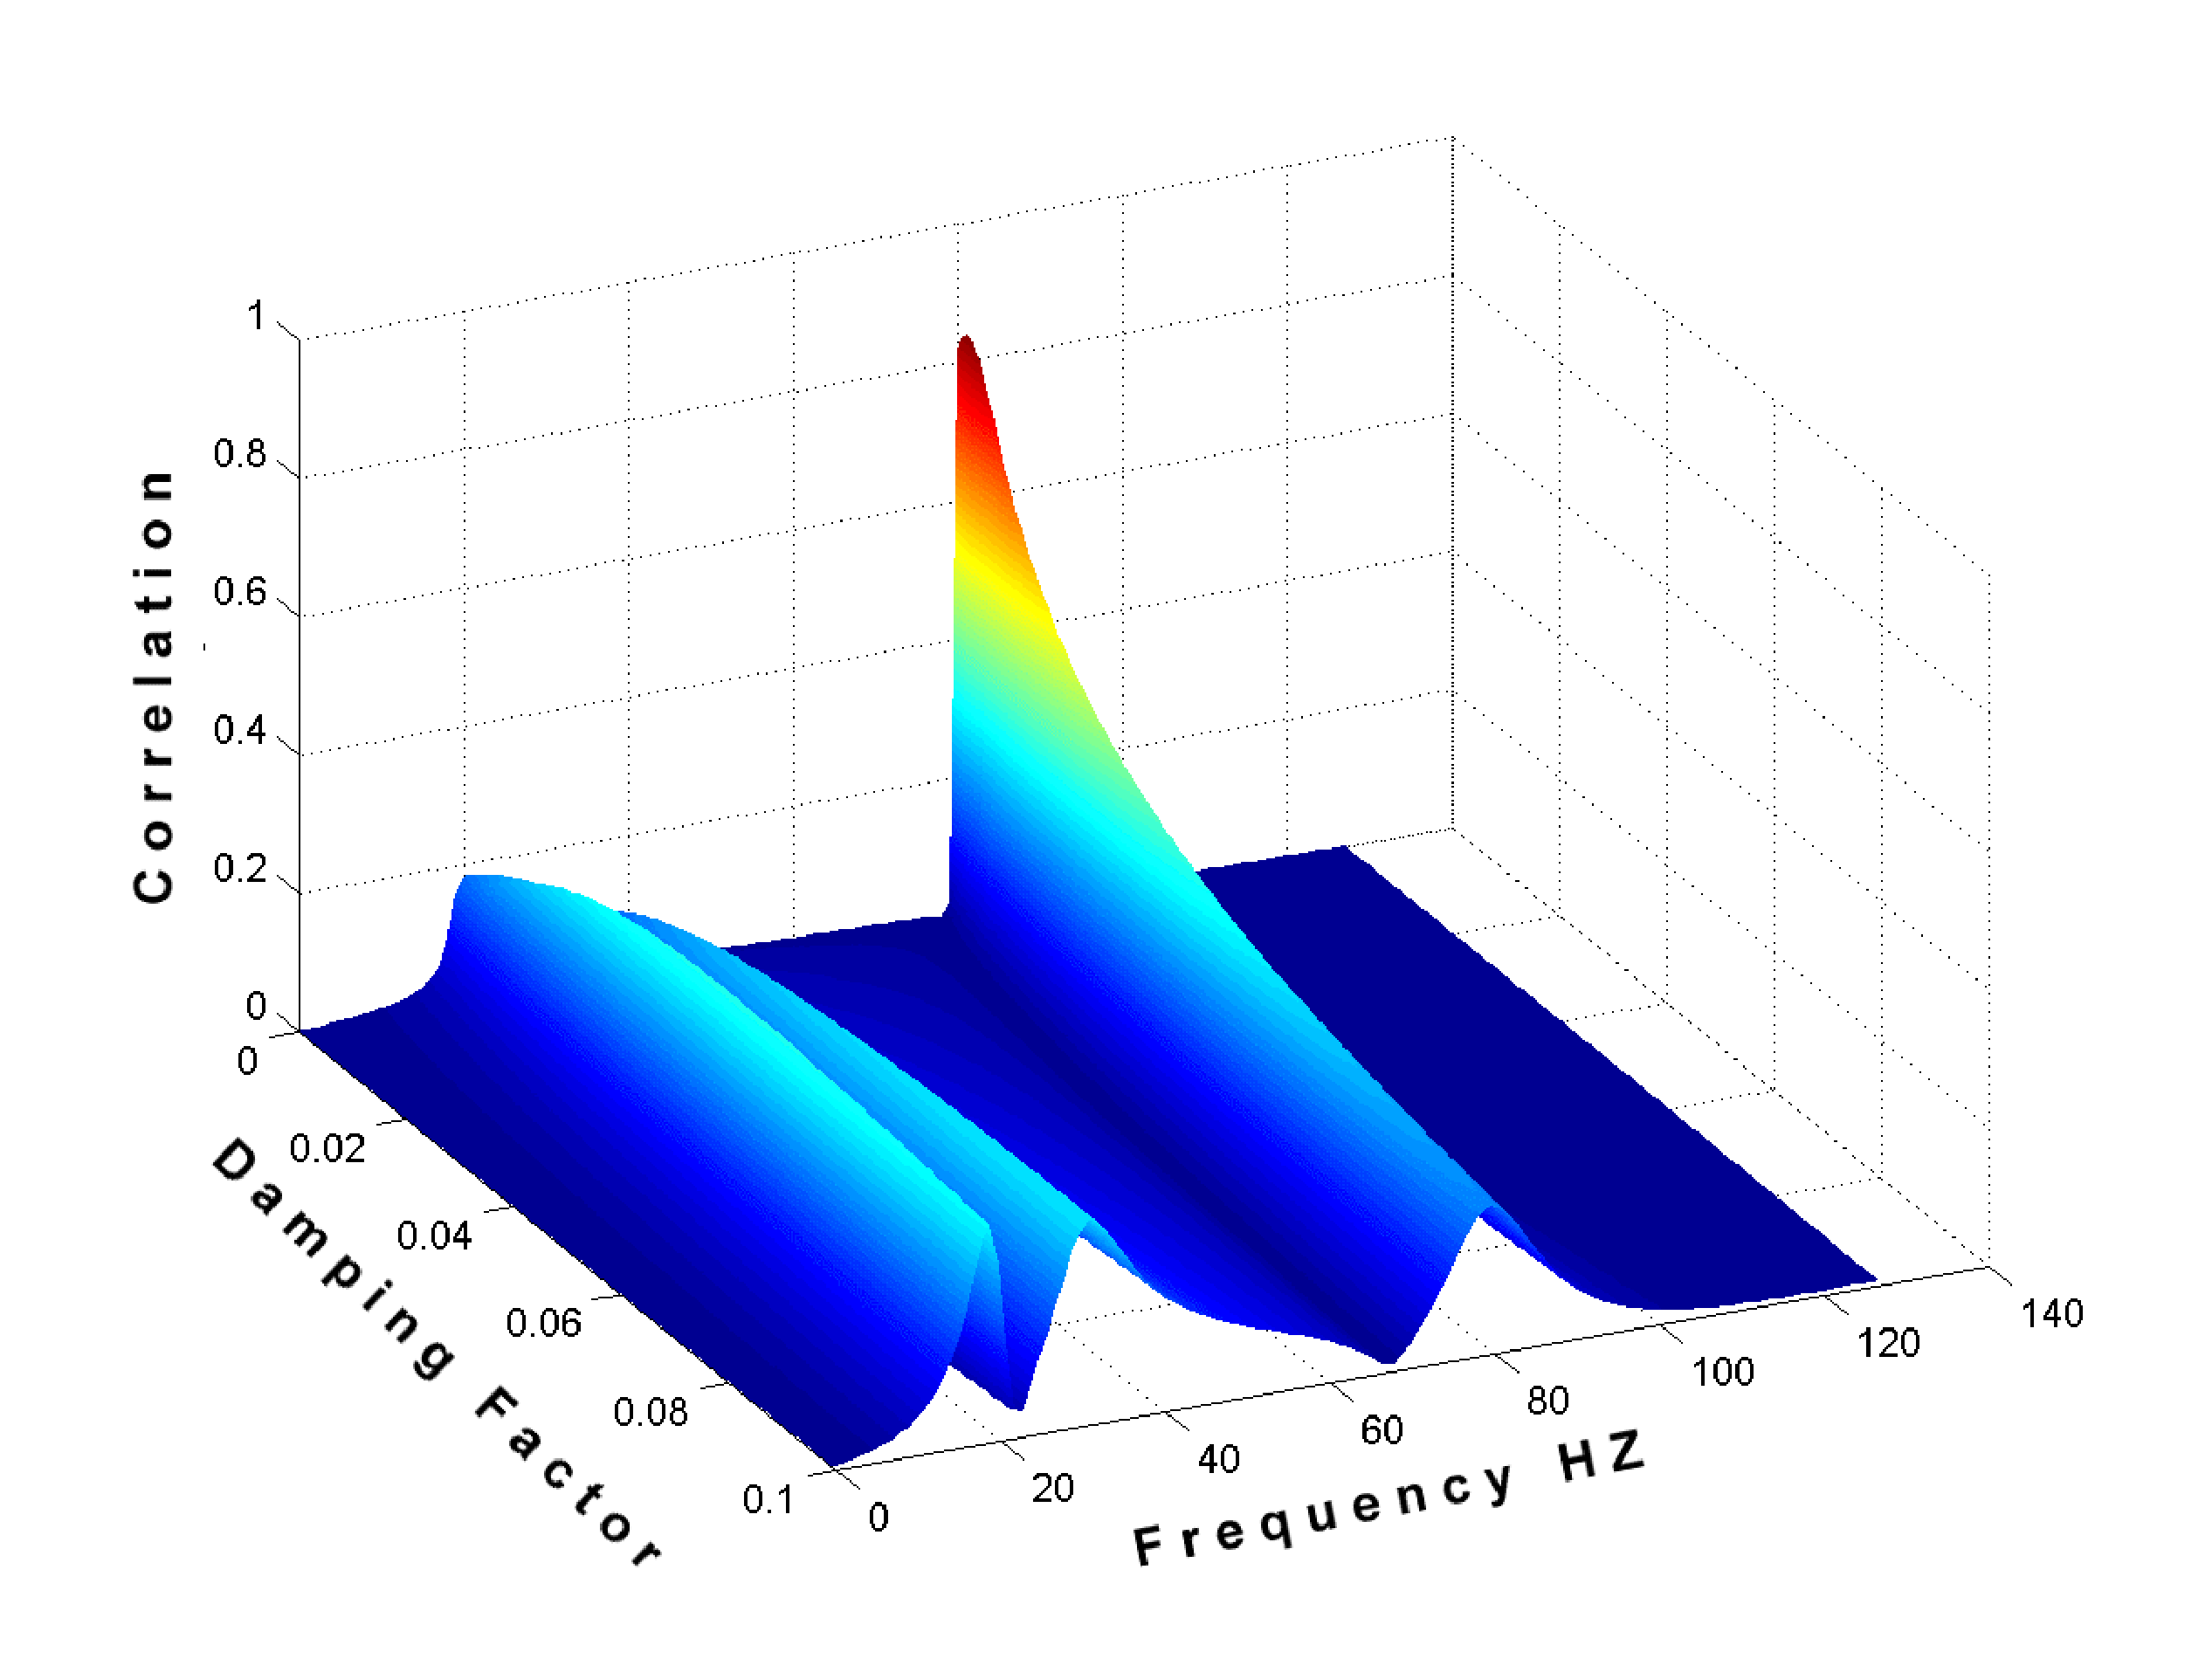
\includegraphics[keepaspectratio=true,scale=0.3]{figuras/fig01.eps}
	\caption{Wavelets correlation coefficients}
\end{figure}

\section{Tabela}

As tabelas devem estar centradas entre margens e identificadas por uma legenda 
alinhada a esquerda, com recuo especial de deslocamento de 1,8 cm, posicionada 
acima da tabela com mostrado nas Tabs. (\ref{tab01}) e (2), a título de 
exemplo. O tamanho das fontes empregadas nos rótulos e anotações usadas nas 
tabelas deve ser compatível com o usado no corpo do texto. Rótulos e anotações 
devem estar em português. Um espaçamento de 11 pts deve ser deixado entre a 
legenda e a tabela, bem como após a tabela. 

As grandezas dimensionais mostradas em cada tabela devem apresentar unidades 
consistentes com o SI. As unidades de cada variável devem ser mostradas apenas 
na primeira linha e/ou coluna da tabela, entre colchetes 

A referência explícita no texto à uma dada tabela deve ser feita como 
\lq\lq Tab. (\ref{tab01})\rq\rq\ quando no meio de uma frase ou como 
\lq\lq Tabela (\ref{tab01})\rq\rq\ quando no início da mesma. Referências 
implícitas a uma dada tabela devem ser feitas entre parênteses como 
\lq\lq (Tab. \ref{tab01}). Para referências a mais de uma tabela as mesmas 
regras devem ser aplicadas usando-se o plural adequadamente. Exemplos:
\begin{itemize}
	\item \lq\lq Após os ensaios experimentais, foram obtidos os resultados 
	mostrados na Tab. (\ref{tab01}), que ...\rq\rq
	\item \lq\lq A Tabela (\ref{tab01}) apresenta os resultados obtidos, onde 
	pode-se observar que ...\rq\rq
	\item As Tabelas (1) a (3) apresentam os resultados obtidos, ...\rq\rq
	\item Verificou-se uma forte dependência entre as variáveis citadas 
	(Tab. \ref{tab01}), comprovando ...\rq\rq
\end{itemize}

Cada tabela deve ser posicionada o mais próxima possível da primeira citação 
feita à mesma no texto, imediatamente após o parágrafo no qual é feita a 
citação, se possível, na mesma página.

\begin{table}[h]
	\centering
	\label{tab01}
	
	\begin{tabular}{ccc}
		\toprule
		\textbf{Processing type} & \textbf{Property 1} (\%) & 
		\textbf{Property 2} $[\mu m]$ \\
		\midrule
		Process 1 & 40.0 & 22.7 \\
		Process 2 & 48.4 & 13.9 \\
		Process 3 & 39.0 & 22.5 \\
		Process 4 & 45.3 & 28.5 \\
		\bottomrule
	\end{tabular}

	\caption{Propriedades obtidades após processamento}
\end{table}

\section{Citação de Referências}

Referencias a outros trabalhos tais como artigos, teses, relatórios, etc. devem 
ser feitas no corpo do texto devem estar de acordo com a norma corrente ABNT 
NBR 6023:2002 (ABNT, 2000), esta ultima baseada nas normas ISO 690:1987:
\begin{itemize}
	\item \lq\lq \cite{bordalo1989}, mostraram que...\rq\rq

	\item \lq\lq Resultados disponíveis em \cite{coimbra1978}, \cite{clark1986} 
	e \cite{sparrow1980}, mostram que...\rq\rq
\end{itemize}

Para referências a trabalhos com até dois autores, deve-se citar o nome de 
ambos os autores, por exemplo: \lq\lq \cite{soviero1997}, mostraram 
que...\rq\rq

